% =====================================================================
% The hourglass mode of Lagrange Q2 with reduced 2x2 shear integration:
% origin, consequences in the code, the fix and its caveats
% Standalone document (project notes, dispersion branch, Nov 2026)
% Compile with: pdflatex hourglass_mode.tex
% =====================================================================
\documentclass[11pt]{article}
\usepackage[a4paper, margin=2.5cm]{geometry}
\usepackage{amsmath, amssymb}
\usepackage{tikz}
\usetikzlibrary{arrows.meta}

\title{The hourglass mode of the Q2 plate element:\\ origin, consequences, fix and caveats}
\author{Project notes, dispersion branch}
\date{November 2026}

\begin{document}
\maketitle

\section{Summary}

The forced-response pipeline discretizes the Reissner--Mindlin (RM) plate with
9-node Lagrange Q2 elements and integrates the shear energy with the reduced
$2\times 2$ Gauss rule. That rule cannot see one particular deformation pattern,
the \emph{hourglass mode}: the stiffness matrix assigns it zero energy although the
continuous RM plate would not. On the free $1 \times 1\,\mathrm{m}$ plate it appears
as a fourth zero-frequency mode next to the three rigid-body modes.
\begin{itemize}
  \item \textbf{Bare plate:} small effect (at most about $1.4\,\mathrm{dB}$ on the
        radiated power, typically far less).
  \item \textbf{Plate with resonators on the lattice:} the in-phase resonator mode
        moves from $1273.1\,\mathrm{Hz}$ to $3059\,\mathrm{Hz}$; the insertion loss
        (IL) changes by up to $3.8\,\mathrm{dB}$ near the upper gap edge.
  \item \textbf{Fix:} full $3\times 3$ shear integration (quadrature degree 4),
        the default on the Bloch cell and, since 2026-11-13, in the forced-response
        runs of \texttt{main.py} and the parameter study. Caveats: possible shear
        locking for thinner plates or coarser meshes, and comparability with older
        $2\times 2$ results.
\end{itemize}

% ---------------------------------------------------------------------
\section{The Q2 element and its weights}

\subsection{Shape functions}
Each element is mapped to the reference square $\xi, \eta \in [-1, 1]$. The nine
nodes sit at $\xi, \eta \in \{-1, 0, +1\}$. The 1D quadratic Lagrange polynomials
\begin{equation}
  \ell_-(\xi) = \tfrac12 \xi(\xi - 1), \qquad
  \ell_0(\xi) = 1 - \xi^2, \qquad
  \ell_+(\xi) = \tfrac12 \xi(\xi + 1)
\end{equation}
are $1$ at their own node and $0$ at the other two. The 2D shape function of node
$(a, b)$, $a, b \in \{-, 0, +\}$, is the product $N_{ab}(\xi, \eta) =
\ell_a(\xi)\,\ell_b(\eta)$. Inside an element
\begin{equation}
  w(\xi, \eta) = \sum_{a,b} w_{ab}\, N_{ab}(\xi, \eta),
\end{equation}
and the same for $\theta_x$ and $\theta_y$ with their own nodal values.

\subsection{The weights}
The \emph{weights} $w_{ab}$ (and the nodal rotations) are the degrees of freedom:
the entries of the vector $q$ that the solver computes, an eigenvector of
$K q = \lambda M q$ or the response of a frequency sweep. Neighboring elements share
the nodes on their common edge, so $w$ is continuous across elements.

The space spanned by the $N_{ab}$ is $Q_2$: every product of $\{1, \xi, \xi^2\}$ and
$\{1, \eta, \eta^2\}$. Any function of that form is represented \emph{exactly} by its
nodal values.

% ---------------------------------------------------------------------
\section{Energies and why the shear term is under-integrated}

The RM strain energy of a plate splits into
\begin{align}
  U_b &= \tfrac12 \int \boldsymbol{\kappa}(\boldsymbol{\theta})^\mathsf{T}\, \mathbf{D}_b\,
         \boldsymbol{\kappa}(\boldsymbol{\theta}) \,\mathrm{d}A
         && \text{bending, depends only on } \nabla\boldsymbol{\theta}, \\
  U_s &= \tfrac12 \int \kappa G h\, |\nabla w - \boldsymbol{\theta}|^2 \,\mathrm{d}A
         && \text{shear}, \ \kappa = 5/6 .
\end{align}
\paragraph{Shear locking.} For a thin plate the shear stiffness $\kappa G h$ is huge
compared with the bending stiffness, so the solution should nearly satisfy the
Kirchhoff constraint $\nabla w = \boldsymbol{\theta}$. Low-order element fields
cannot satisfy it exactly everywhere; with exact integration the leftover shear
strain costs spurious energy and the element becomes too stiff (``locks''). The
classical remedy is \emph{reduced integration}: evaluate $U_s$ with fewer quadrature
points, so the constraint only needs to hold at those points. For Q2 that is the
$2\times 2$ rule (\texttt{weak\_form.py}: quadrature degree $2\cdot\mathrm{deg} - 2 = 2$).

\subsection{Gauss rules}
An $n$-point Gauss rule integrates polynomials up to degree $2n - 1$ exactly.
\begin{center}
\begin{tabular}{|l|l|l|l|}
\hline
Rule & Points per direction & Weights & Exact up to degree \\
\hline
$2\times 2$ & $\pm 1/\sqrt{3} \approx \pm 0.577$ & $1, 1$ & 3 \\
$3\times 3$ & $0,\ \pm\sqrt{3/5} \approx \pm 0.775$ & $8/9,\ 5/9$ & 5 \\
\hline
\end{tabular}
\end{center}
The $3\times 3$ points are \emph{not} the nodes $\{-1, 0, 1\}$: that would be the
Gauss--Lobatto (Simpson) rule.

\begin{figure}[htbp]
\centering
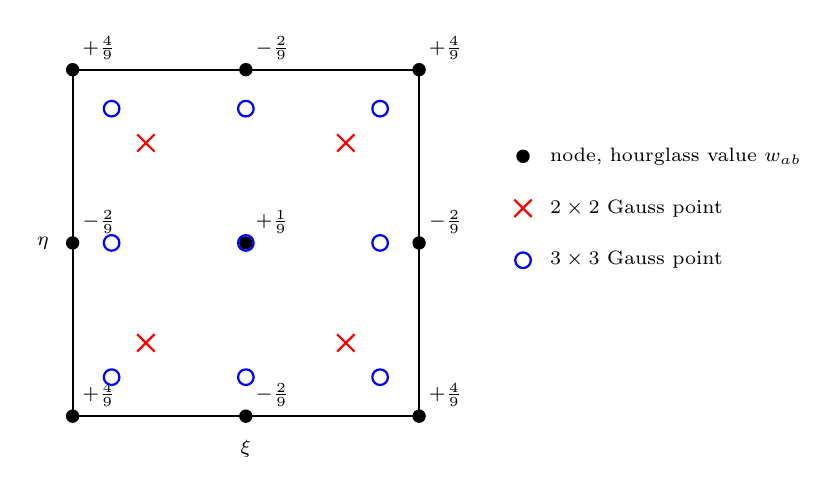
\begin{tikzpicture}[scale=2.2]
  \draw[thick] (-1,-1) rectangle (1,1);
  % nodes with hourglass nodal values
  \foreach \x in {-1,1} \foreach \y in {-1,1} {
    \fill (\x,\y) circle (1.1pt);
    \node[font=\scriptsize, anchor=south west] at (\x,\y) {$+\frac49$};
  }
  \foreach \p in {(-1,0),(1,0),(0,-1),(0,1)} {
    \fill \p circle (1.1pt);
    \node[font=\scriptsize, anchor=south west] at \p {$-\frac29$};
  }
  \fill (0,0) circle (1.1pt);
  \node[font=\scriptsize, anchor=south west] at (0,0) {$+\frac19$};
  % 2x2 Gauss points (crosses)
  \foreach \x in {-0.577,0.577} \foreach \y in {-0.577,0.577} {
    \draw[red, thick] (\x-0.05,\y-0.05) -- (\x+0.05,\y+0.05);
    \draw[red, thick] (\x-0.05,\y+0.05) -- (\x+0.05,\y-0.05);
  }
  % 3x3 Gauss points (open circles)
  \foreach \x in {-0.775,0,0.775} \foreach \y in {-0.775,0,0.775} {
    \draw[blue, thick] (\x,\y) circle (0.045);
  }
  \node[font=\scriptsize, below] at (0,-1.08) {$\xi$};
  \node[font=\scriptsize, left] at (-1.08,0) {$\eta$};
  % legend
  \begin{scope}[xshift=1.6cm, yshift=0.5cm]
    \fill (0,0) circle (1.1pt); \node[font=\scriptsize, right] at (0.1,0) {node, hourglass value $w_{ab}$};
    \draw[red, thick] (-0.05,-0.35) -- (0.05,-0.25); \draw[red, thick] (-0.05,-0.25) -- (0.05,-0.35);
    \node[font=\scriptsize, right] at (0.1,-0.3) {$2\times 2$ Gauss point};
    \draw[blue, thick] (0,-0.6) circle (0.045); \node[font=\scriptsize, right] at (0.1,-0.6) {$3\times 3$ Gauss point};
  \end{scope}
\end{tikzpicture}
\caption{Reference element: the 9 nodes (with the nodal values of the hourglass
pattern), the 4 points of the $2\times 2$ rule and the 9 points of the $3\times 3$
rule.}
\label{fig:element}
\end{figure}

% ---------------------------------------------------------------------
\section{The hourglass pattern}

\subsection{Construction}
Take
\begin{equation}
  w = P(\xi)\,P(\eta), \qquad P(s) = s^2 - \tfrac13, \qquad \boldsymbol{\theta} = 0 .
\end{equation}
$P$ is, up to a factor, the Legendre polynomial $P_2(s) = (3s^2 - 1)/2$, whose roots
are exactly the two Gauss points $\pm 1/\sqrt{3}$ (Figure~\ref{fig:factor}). The
pattern lies in $Q_2$, so the element represents it exactly. Its nodal values are
\begin{center}
\begin{tabular}{|l|l|l|}
\hline
Node type & $(\xi, \eta)$ & $w_{ab}$ \\
\hline
element corner & $(\pm 1, \pm 1)$ & $(\tfrac23)(\tfrac23) = +4/9$ \\
mid-side & $(\pm 1, 0)$, $(0, \pm 1)$ & $(\tfrac23)(-\tfrac13) = -2/9$ \\
element center & $(0, 0)$ & $(-\tfrac13)(-\tfrac13) = +1/9$ \\
\hline
\end{tabular}
\end{center}
In 1D: $P(s) = \tfrac23\,\ell_-(s) - \tfrac13\,\ell_0(s) + \tfrac23\,\ell_+(s)$.

\begin{figure}[htbp]
\centering
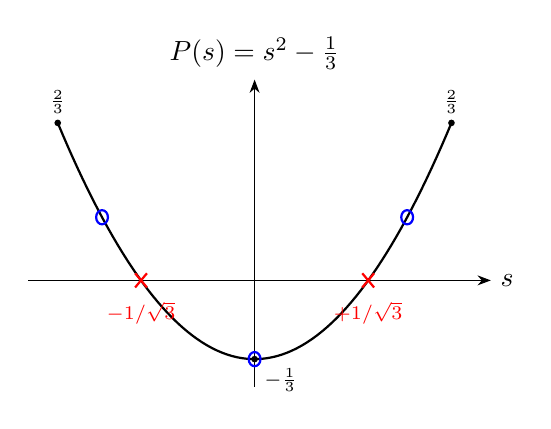
\begin{tikzpicture}[x=2.5cm, y=3cm, >={Stealth}]
  \draw[->] (-1.15,0) -- (1.2,0) node[right] {$s$};
  \draw[->] (0,-0.45) -- (0,0.85) node[above] {$P(s) = s^2 - \frac13$};
  \draw[thick] plot[domain=-1:1, samples=80] (\x, {\x*\x - 1/3});
  \foreach \s in {-0.577,0.577} {
    \draw[red, thick] (\s-0.03,-0.03) -- (\s+0.03,0.03);
    \draw[red, thick] (\s-0.03,0.03) -- (\s+0.03,-0.03);
  }
  \node[red, font=\scriptsize, below] at (0.577,-0.05) {$+1/\sqrt3$};
  \node[red, font=\scriptsize, below] at (-0.577,-0.05) {$-1/\sqrt3$};
  \foreach \s in {-0.775,0,0.775} \draw[blue, thick] (\s,{\s*\s-1/3}) circle (0.03);
  \foreach \s in {-1,1} { \fill (\s,2/3) circle (1.2pt); \node[font=\scriptsize, above] at (\s,2/3) {$\frac23$}; }
  \fill (0,-1/3) circle (1.2pt); \node[font=\scriptsize, below right] at (0,-1/3) {$-\frac13$};
\end{tikzpicture}
\caption{The 1D factor $P(s)$. It vanishes at the $2\times 2$ Gauss points (red),
but not at any of the $3\times 3$ points (blue circles): $P(0) = -\frac13$,
$P(\pm 0.775) = \frac{4}{15}$. Dots: nodal values.}
\label{fig:factor}
\end{figure}

\subsection{What each rule sees}
With $\boldsymbol{\theta} = 0$ the bending energy is zero, and the shear strain is
$\nabla w$:
\begin{equation}
  \frac{\partial w}{\partial \xi} = 2\xi\, P(\eta), \qquad
  \frac{\partial w}{\partial \eta} = 2\eta\, P(\xi), \qquad
  |\nabla w|^2 = 4\xi^2 P(\eta)^2 + 4\eta^2 P(\xi)^2 .
\end{equation}
Each derivative is the derivative of one factor \emph{times the other factor}, and
at a $2\times 2$ point the other factor vanishes. So at those points both the
displacement and the slope are zero.
\begin{center}
\begin{tabular}{|l|l|l|l|l|l|}
\hline
Rule & Point $(\xi, \eta)$ & Weight & $w$ & $(\partial_\xi w, \partial_\eta w)$ & $|\nabla w|^2$ \\
\hline
$2\times 2$ & $(\pm 0.577, \pm 0.577)$, 4 points & $1$ & $0$ & $(0, 0)$ & $\mathbf{0}$ \\
\hline
$3\times 3$ & $(0, 0)$ & $64/81$ & $+1/9$ & $(0, 0)$ & $0$ \\
$3\times 3$ & $(\pm 0.775, 0)$, 2 points & $40/81$ & $-4/45$ & $(\mp 0.516, 0)$ & $\mathbf{0.267}$ \\
$3\times 3$ & $(0, \pm 0.775)$, 2 points & $40/81$ & $-4/45$ & $(0, \mp 0.516)$ & $\mathbf{0.267}$ \\
$3\times 3$ & $(\pm 0.775, \pm 0.775)$, 4 points & $25/81$ & $+16/225$ & $(\pm 0.413, \pm 0.413)$ & $\mathbf{0.341}$ \\
\hline
\end{tabular}
\end{center}
Sums (reference element, factor $\kappa G h$ and Jacobian omitted):
\begin{itemize}
  \item $2\times 2$: $4 \cdot 1 \cdot 0 = 0$. The matrix assigns \emph{zero} shear energy.
  \item $3\times 3$: $4 \cdot \tfrac{40}{81} \cdot 0.267 + 4 \cdot \tfrac{25}{81} \cdot 0.341
        = 0.948$, equal to the exact integral $128/135$ (the integrand has degree 4 per
        direction, $\le 5$). On the production mesh this gives a frequency of
        about $498\,\mathrm{kHz}$.
\end{itemize}
What matters is the \emph{strain}, not the displacement: rigid translation
($w = $ const) has nonzero displacement and zero strain everywhere and is a genuine
zero mode; a pattern that vanishes at the Gauss points but is tilted there would still
cost energy.

\subsection{Why it is a zero mode and not a coincidence}
\paragraph{One pattern, copied into every element.} Every element carries the same
function, so if it has zero strain at the four Gauss points of one element, it has
zero strain in all of them. On a shared edge ($\xi = \pm 1$) both neighbors give
$w = \tfrac23 P(\eta)$, so the global field is continuous (Figure~\ref{fig:side_view}).
The global vector is simply $+4/9$ on every element-corner node, $-2/9$ on every
mid-side node, $+1/9$ on every element-center node, and $0$ for all rotations.

\begin{figure}[htbp]
\centering
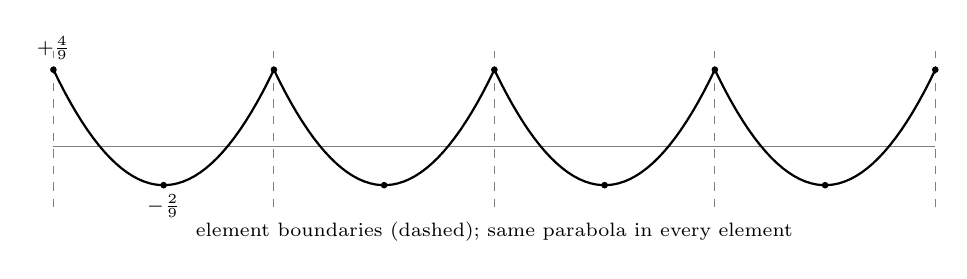
\begin{tikzpicture}[x=1.4cm, y=2.2cm]
  \draw[gray] (0,0) -- (8,0);
  \foreach \e in {0,1,2,3} {
    \draw[thick] plot[domain=0:2, samples=40] ({2*\e + \x}, {(2/3)*((\x-1)*(\x-1) - 1/3)});
    \draw[gray, dashed] (2*\e,-0.35) -- (2*\e,0.55);
    \fill (2*\e,4/9) circle (1.2pt);
    \fill (2*\e+1,-2/9) circle (1.2pt);
  }
  \draw[gray, dashed] (8,-0.35) -- (8,0.55);
  \fill (8,4/9) circle (1.2pt);
  \node[font=\scriptsize, above] at (0,4/9) {$+\frac49$};
  \node[font=\scriptsize, below] at (1,-2/9) {$-\frac29$};
  \node[font=\scriptsize, below] at (4,-0.38) {element boundaries (dashed); same parabola in every element};
\end{tikzpicture}
\caption{Side view of the hourglass pattern along a line of element edges
($\eta = \pm 1$): $w = \frac23 P(\xi)$ repeated in every element, continuous at the
shared nodes.}
\label{fig:side_view}
\end{figure}

\paragraph{The eigensolver looks for it.} With the quadrature the shear energy
becomes a quadratic form $U(q) = \frac12 q^\mathsf{T} K q$. Picture $U$ as a bowl over
the space of all nodal vectors $q$: elastic deformations go uphill in every direction,
a zero mode is a direction in which the bowl is flat, $q^\mathsf{T} K q = 0$. Whether
such a direction exists is a property of $K$, fixed by mesh and quadrature rule. The
eigensolver returns the vectors with the smallest Rayleigh quotient
$q^\mathsf{T} K q / q^\mathsf{T} M q$, so it finds every flat direction.

\paragraph{Why the frequency is zero and not undefined.} The mass matrix is integrated
exactly, so the kinetic energy $\frac12\omega^2 \int \rho h\, w^2\,\mathrm{d}A$ of the
pattern is nonzero: stiffness over mass is $0/(\text{positive}) = 0$. The pattern
moves; it costs nothing.

\paragraph{Why ``hourglass''.} The name comes from the 4-node element, whose spurious
mode deforms the square into an hourglass shape. It is used for every
zero-energy mode created by under-integration.

% ---------------------------------------------------------------------
\section{Consequences in the code}

\subsection{Bloch cell (found on Day 2, fixed then)}
The pattern is identical in every element, so it fits any periodic cell: at $\Gamma$
it is a second zero mode, and away from $\Gamma$ it forms a spurious branch that runs
through the spectrum (about $7148\,\mathrm{Hz}\cdot|\mathbf{k}|L/\pi$ on the
$1\,\mathrm{m}$ test cell). \textbf{Fix applied then:} full $3\times 3$ shear
integration is the default of \texttt{assemble\_unit\_cell\_matrices}. The FE bands
then lie at most $0.33\,\%$ above the analytic RM bands below $5\,\mathrm{kHz}$ at
$100$ elements per meter. \texttt{test\_periodic\_reduction.py} still uses $2\times 2$
and therefore expects two zero modes at $\Gamma$.

\subsection{Free finite plate, bare (open check (a))}
The forced-response pipeline (Lagrange Q2, $2\times 2$ shear) gives four
zero-frequency modes on the free $1 \times 1\,\mathrm{m}$ plate. Check (a) showed:
\begin{itemize}
  \item the hourglass vector has Rayleigh quotient $\approx 0$ with $2\times 2$ and lies
        $100\,\%$ in the zero-mode space; with $3\times 3$ there are exactly three zero
        modes and the elastic modes change by at most $0.03\,\%$;
  \item driving-point mobility of the shaker into the hourglass: $0.31$ of that into
        rigid translation;
  \item at the element centers, where the radiated power is evaluated, every element
        shows $+1/9$: the radiation calculation sees a uniform piston, although the
        true mean displacement over an element is zero
        ($\int_{-1}^{1} P(s)\,\mathrm{d}s = 0$);
  \item share of the radiated power: $-30\,\mathrm{dB}$ median, at most
        $-15\,\mathrm{dB}$ (at $500\,\mathrm{Hz}$), i.e.\ at most about
        $1.4\,\mathrm{dB}$ on the bare power.
\end{itemize}

\subsection{Finite plate with resonators}
The resonators sit on element corners, where the pattern is largest ($+4/9$; in the
normalized mode $0.798$ at the attachment points).
\begin{itemize}
  \item When all resonators move in phase they push the plate in the hourglass pattern,
        which the plate can follow at zero stiffness and with little mass moving per
        unit corner motion. The resonators effectively stand on a much lighter base,
        and a resonator on a light base has a frequency well above $f_r$,
        $f \approx f_r\sqrt{1 + m_\mathrm{res}/m_\mathrm{base}}$.
  \item Result: the in-phase resonator mode moves from $1273.1\,\mathrm{Hz}$ ($3\times 3$,
        matching the Bloch value $1273.5\,\mathrm{Hz}$ at $\Gamma$) to
        $3059\,\mathrm{Hz}$ ($2\times 2$; hourglass participation $0.655$). A
        three-mass estimate gave $3286\,\mathrm{Hz}$ ($7\,\%$ too high). Every
        resonator pattern with a nonzero sum is shifted up in the same way.
  \item Effect on the IL, $900$--$1500\,\mathrm{Hz}$ (check (c)):
\end{itemize}
\begin{center}
\begin{tabular}{|l|l|l|l|}
\hline
Shear rule & IL peak & IL dip & IL changes sign at \\
\hline
$2\times 2$ (pipeline) & $+12.9\,\mathrm{dB}$ at $1115\,\mathrm{Hz}$ & $-13.9\,\mathrm{dB}$ at $1257\,\mathrm{Hz}$ & $\approx 1180\,\mathrm{Hz}$, inside the gap \\
$3\times 3$ & $+13.0\,\mathrm{dB}$ at $1120\,\mathrm{Hz}$ & $-13.9\,\mathrm{dB}$ at $1267\,\mathrm{Hz}$ & $\approx 1197\,\mathrm{Hz}$, upper gap edge ($1195\,\mathrm{Hz}$) \\
\hline
\end{tabular}
\end{center}
Mean difference $+0.19\,\mathrm{dB}$, maximum $3.8\,\mathrm{dB}$ at $1180\,\mathrm{Hz}$.
With $3\times 3$ the IL is positive across the whole Bloch gap, as the Bloch picture
predicts. The radiation explanation of the dip holds with both rules (cluster
$\sigma = 0.35$--$0.90$ with $2\times 2$, $0.54$--$0.80$ with $3\times 3$).

\paragraph{All three tunings with both rules.} Equal-force radiated-power IL, $10 \times 10$
resonators, $\mu = 0.25$ (\texttt{check\_finite\_plate\_modes.py insertion\_loss\_all}):
\begin{center}
\begin{tabular}{|l|l|l|l|l|}
\hline
$f_r$, Bloch gap & Rule & IL peak & mean IL in gap & IL $< 0$ in gap \\
\hline
$600\,\mathrm{Hz}$, $578$--$662\,\mathrm{Hz}$ & $2\times 2$ & $+16.5\,\mathrm{dB}$ at $591\,\mathrm{Hz}$ & $+3.7\,\mathrm{dB}$ & from $630\,\mathrm{Hz}$ ($38\,\%$) \\
 & $3\times 3$ & $+22.2\,\mathrm{dB}$ at $594\,\mathrm{Hz}$ & $+5.6\,\mathrm{dB}$ & from $633\,\mathrm{Hz}$ ($35\,\%$) \\
$1200\,\mathrm{Hz}$, $1031$--$1194\,\mathrm{Hz}$ & $2\times 2$ & $+12.9\,\mathrm{dB}$ at $1115\,\mathrm{Hz}$ & $+8.6\,\mathrm{dB}$ & from $1184\,\mathrm{Hz}$ ($8\,\%$) \\
 & $3\times 3$ & $+13.0\,\mathrm{dB}$ at $1120\,\mathrm{Hz}$ & $+9.4\,\mathrm{dB}$ & none \\
$2000\,\mathrm{Hz}$, no gap & $2\times 2$ & $+6.4\,\mathrm{dB}$ at $2054\,\mathrm{Hz}$ & -- & -- \\
 & $3\times 3$ & $+6.3\,\mathrm{dB}$ at $2063\,\mathrm{Hz}$ & -- & -- \\
\hline
\end{tabular}
\end{center}
Largest differences between the rules: $5.7\,\mathrm{dB}$ at $594\,\mathrm{Hz}$,
$3.8\,\mathrm{dB}$ at $1180\,\mathrm{Hz}$, $1.8\,\mathrm{dB}$ at $2316\,\mathrm{Hz}$; mean
differences $+0.1$ to $+0.2\,\mathrm{dB}$. The negative IL in the upper part of the
$600\,\mathrm{Hz}$ gap is therefore \emph{not} the artifact: it remains with $3\times 3$.
Its cause is radiation (theory notes, Chapter~9). Split into the two terms of the IL
($3\times 3$, averages over the band):
\begin{center}
\begin{tabular}{|l|l|l|l|}
\hline
Band & IL & velocity term & efficiency term \\
\hline
$600\,\mathrm{Hz}$ case, $578$--$628\,\mathrm{Hz}$ & $+13.7\,\mathrm{dB}$ & $+20.1\,\mathrm{dB}$ & $-6.4\,\mathrm{dB}$ \\
$600\,\mathrm{Hz}$ case, $628$--$662\,\mathrm{Hz}$ & $-7.4\,\mathrm{dB}$ & $+7.8\,\mathrm{dB}$ & $-15.2\,\mathrm{dB}$ \\
$1200\,\mathrm{Hz}$ case, $1031$--$1129\,\mathrm{Hz}$ & $+10.6\,\mathrm{dB}$ & $+13.8\,\mathrm{dB}$ & $-3.2\,\mathrm{dB}$ \\
$1200\,\mathrm{Hz}$ case, $1129$--$1194\,\mathrm{Hz}$ & $+7.3\,\mathrm{dB}$ & $+10.0\,\mathrm{dB}$ & $-2.7\,\mathrm{dB}$ \\
\hline
\end{tabular}
\end{center}
The plate still moves less in the upper part of the $600\,\mathrm{Hz}$ gap, but it
radiates $15\,\mathrm{dB}$ more efficiently than the bare plate. Two reasons: there the
upper gap edge is the resonator band at $\Gamma$ (regime~1 in Section~5.11 of the theory notes, $\tau = 0.5$), whose small-$k$ plate motion is
supersonic, while at $1200\,\mathrm{Hz}$ it is the sin pattern at $X$
($k = \pi/a = 31.4\,\mathrm{rad/m}$ against $k_\mathrm{air} = 21.9\,\mathrm{rad/m}$ at
$1194\,\mathrm{Hz}$), which is subsonic; and at $600\,\mathrm{Hz}$ the bare plate is
four times below its critical frequency and radiates even worse.

% ---------------------------------------------------------------------
\section{The fix}

Full $3\times 3$ shear integration (quadrature degree 4) removes the flat direction:
the $3\times 3$ rule integrates the shear energy of Q2 fields exactly, so $K$ is the
exact Galerkin matrix of the RM operator and every zero mode of $K$ is a genuine
rigid-body mode. The FE eigenvalues are again Rayleigh--Ritz upper bounds of the
continuous ones.

\paragraph{Implementation (defaults keep $2\times 2$).}
\begin{itemize}
  \item \texttt{define\_weak\_form(..., shear\_quadrature\_degree=None)}: \texttt{None}
        keeps $2\times 2$; \texttt{4} gives $3\times 3$.
  \item \texttt{frequency\_sweep\_plate(..., shear\_quadrature\_degree=None)} passes it on.
  \item \texttt{FinitePlateSetup.shear\_quadrature\_degree}: enters the cache key only
        when set, so the $2\times 2$ caches stay valid.
  \item \texttt{solve\_evp(..., shear\_quadrature\_degree=None)} (added 2026-11-13).
\end{itemize}
\paragraph{Applied (2026-11-13).} \texttt{main.py} sets
\texttt{shear\_quadrature\_degree = 4} and passes it to the eigenfrequency solves, both
sweeps and the parameter-study setup; it enters the eigenfrequency and sweep cache keys
only when set. Rebuilt: bare and resonator sweeps $500$--$5000\,\mathrm{Hz}$
($578$ frequencies each), the $600$ and $2000\,\mathrm{Hz}$ windows, both eigenfrequency
sets ($500$ modes). The free bare plate now has exactly three zero modes, the plate
with resonators as well. The forced-response validations were rerun with $3\times 3$
(option \texttt{--full-shear}): reciprocity, passivity and radiation pass; the
eigenvalue validation gives the same verdicts as with $2\times 2$ (one case fails with
both rules, $2.21\,\%$ below its reference instead of $2.28\,\%$).


% ---------------------------------------------------------------------
\section{Caveats of the fix}

\begin{center}
\begin{tabular}{|p{0.28\textwidth}|p{0.62\textwidth}|}
\hline
Caveat & Status \\
\hline
Shear locking & The reason reduced integration exists. At the production mesh not an
issue: on the $1\times 1\,\mathrm{m}$ plate the elastic modes move up by at most
$0.07\,\%$ below $1\,\mathrm{kHz}$, $0.13\,\%$ below $2\,\mathrm{kHz}$ and $0.32\,\%$
below $5\,\mathrm{kHz}$ (mean $0.12\,\%$; the earlier ``$0.03\,\%$'' held only for the
lowest modes); the Bloch cell at $100$ elements per meter is within $0.33\,\%$ of the
analytic bands. Locking grows for
thinner plates and coarser meshes: rerun a mesh check for every new thickness,
material or mesh (fixed elements-per-meter values do not transfer between
thicknesses). \\
\hline
Cost & Assembly is slightly more expensive, the solve dominates: negligible per
frequency. The cache rebuild is the real cost (about $50\,\mathrm{min}$ per sweep). \\
\hline
Comparability & Results committed before 2026-11-13 (forced response, parameter
study) used $2\times 2$; the figures are now regenerated with $3\times 3$. The $2\times 2$
caches remain and are reached with \texttt{shear\_quadrature\_degree = None}. \\
\hline
Validation & Rerun with $3\times 3$: passes (see above). \\
\hline
Serendipity & Not checked; the pipeline uses Lagrange. \\
\hline
Other remedies & Selective reduced integration with hourglass stabilization, or
mixed/assumed-strain elements (e.g.\ MITC), avoid both locking and spurious modes.
Not pursued: $3\times 3$ is sufficient at the current mesh and thickness. \\
\hline
Point-force singularity & Unaffected: the slow drift of the resonator band with mesh
refinement ($1273.5$ / $1271.7$ / $1270.5\,\mathrm{Hz}$) is a property of the RM plate
under a point force, not of the quadrature. \\
\hline
\end{tabular}
\end{center}

\end{document}
